% These are the lecture notes for my CSCI360 course SPRING 2017
% at John Jay College of Criminal Justice. They are based largely on
% Schneier's Applied Cryptography.

% Feel free to edit these slides and use them for your own courses.
% HOWEVER DO NOT REMOVE THESE LINES!
% Email me at: awood [at] jjay.cuny.edu
% or at: awood [at] gradcenter.cuny.edu


\documentclass{beamer}

\usepackage{tikz}
\usetikzlibrary{calc}

\usepackage{forest}
\usepackage{verbatim}
\usepackage{color}
\usepackage{amsmath}
\usepackage{graphicx}
\usepackage{caption}



\setbeamertemplate{footline}[frame number]
\setbeamertemplate{navigation symbols}{} 

\newtheorem{thm}{Theorem}[section]
\newtheorem{lem}{Lemma}
\newtheorem{cl}{Claim}
\newtheorem{cor}{Corollary}[section]
\newtheorem{conj}{Conjecture}
\newtheorem{quest}{Question}
\newtheorem{defn}{Definition}[section]
\newtheorem{obs}{Observation}[section]
\newtheorem{exam}{Example}

\newcommand{\im}{\operatorname{im}}
\newcommand{\id}{\operatorname{id}}
\newcommand{\interior}{\operatorname{int}}
\newcommand{\bdry}{\operatorname{bdry}}
\newcommand{\<}{\langle}
\renewcommand{\>}{\rangle}
\newcommand{\Gab}{(G_\phi)^{ab}} 
\newcommand{\phibar}{\bar{\phi}}
\newcommand{\Z}{\mathbb{Z}}
\newcommand{\N}{\mathbb{N}}
\newcommand{\Q}{\mathbb{Q}}
\newcommand{\R}{\mathbb{R}}
\newcommand{\C}{\mathbb{C}}
\newcommand{\A}{\mathcal{A}}
\newcommand{\OO}{\mathcal{O}}
\newcommand{\UU}{\mathcal{U}}
\newcommand{\power}{2^{\{P_1, \cdots , P_n\}}}
\newcommand{\bp}{\begin{problem}}
\newcommand{\ep}{\end{problem}}
\newcommand{\ba}{\begin{answer}}
\newcommand{\ea}{\end{answer}}
\newcommand{\ds}{\displaystyle}
\newcommand{\ben}{\renewcommand{\theenumi}{\alph{enumi}}
\renewcommand{\labelenumi}{(\theenumi)}\begin{enumerate}}
\newcommand{\een}{\end{enumerate}}
\newcommand{\Hess}{\operatorname{Hessian}}
\newcommand{\Aut}{\mathrm{Aut}}
\newcommand{\Inn}{\mathrm{Inn}}
\newcommand{\Out}{\mathrm{Out}}
\newcommand{\End}{\mathrm{End}}


\mode<presentation>
{
%  \usetheme{default}
  \setbeamercovered{invisible}
}


\usepackage[english]{babel}
\usepackage[latin1]{inputenc}
\usepackage{times}
\usepackage[T1]{fontenc}
\usepackage{stmaryrd}

%\usetheme{default}
%\usetheme{AnnArbor}
%\usetheme{Antibes}
%\usetheme{Bergen}
%\usetheme{Berkeley}
%\usetheme{Berlin}
%\usetheme{Boadilla}
%\usetheme{CambridgeUS}
%\usetheme{Copenhagen}
%\usetheme{Darmstadt}
%\usetheme{Dresden}
%\usetheme{Frankfurt}
%\usetheme{Goettingen}
%\usetheme{Hannover}
%\usetheme{Ilmenau}
%\usetheme{JuanLesPins}
%\usetheme{Luebeck}
%\usetheme{Madrid}
%\usetheme{Malmoe}
%\usetheme{Marburg}
%\usetheme{Montpellier}
%\usetheme{PaloAlto}
%\usetheme{Pittsburgh}
%\usetheme{Rochester}
\usetheme{Singapore}
%\usetheme{Szeged}
%\usetheme{Warsaw}

%\usecolortheme{default}
%\usecolortheme{albatross}
\usecolortheme{beaver}
%\usecolortheme{beetle}
%\usecolortheme{crane}
%\usecolortheme{dolphin}
%\usecolortheme{dove} % grey, white, yellow
%\usecolortheme{fly} %grey, yellow
%\usecolortheme{lily} %white, yellow, blue
%\usecolortheme{orchid}
%\usecolortheme{rose}
%\usecolortheme{seagull}
%\usecolortheme{seahorse}
%\usecolortheme{whale}
%\usecolortheme{wolverine}

% Title page

\title[HF]{Hash Functions}

\subtitle{Based on \emph{Applied Cryptography} by Schneier, Chapter 18}

\author
{Lecture notes of Alexander Wood \\ \scriptsize \href{mailto:awood@jjay.cuny.edu}{awood@jjay.cuny.edu}}
\institute[JJay]{John Jay College of Criminal Justice}  

\date{}

\begin{document}

% Remove 'figure' text from figure captions 
\setbeamertemplate{caption}{\raggedright\insertcaption\par}

\begin{frame}
  \titlepage
\end{frame}

\begin{frame}
\frametitle{Hashing}

A \textbf{hash function}, informally, is a method of taking a numerical input of one value and returning a compressed numerical input of a fixed (smaller) length. 
\end{frame}

\begin{frame}
\frametitle{Why Hash, generally?}

In modern days, there is truly a massive amount of content being generated by users all over the world every day.\newline

Simply in terms of data storage, why will traditional data structures such as arrays and linked lists no longer operate efficiently?
\end{frame}

\begin{frame}
\frametitle{Why Hash, generally?}

These methods of data storage can take data retrieval time of linear order $\mathcal O(n)$. By \textbf{hashing} the values we can retrieve data in only linear time $\mathcal O (1)$.
\end{frame}


\begin{frame}
\frametitle{Why Hash... In Cryptography?}

\textbf{Cryptographic hash functions} are a main feature of modern cryptography. 
\begin{figure}
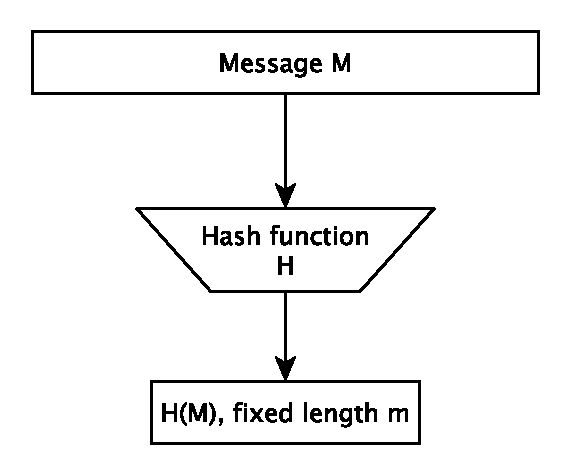
\includegraphics[scale=.6]{IMG/hash.pdf}
\end{figure}
\end{frame}


\begin{frame}
\frametitle{Hash Functions}

A \textbf{one-way hash function} $H(M)$ takes as input a message $M$ of arbitrary length. It returns a value $h$ of fixed length $m$ called a \textbf{hash value}.
\end{frame}

\begin{frame}
\frametitle{Vocab!}

\begin{itemize}
\item The process of converting data from an arbitrary length to a fixed length is called \textbf{hashing} the data.
\item Hash functions are sometimes referred to as \textbf{compression functions}, since the fixed length output is in most applications smaller than the input values.
\item The hash of a large data value is referred to as a \textbf{digest}.
\item If the fixed length of the output of a hash function is $m$ bits, we call $H$ an \textbf{$m$-bit hash function}.
\end{itemize}
\end{frame}


\begin{frame}
\frametitle{Hash Function Properties}

A one-way hash function must satisfy the following properties:
\begin{itemize}
\item Given $M$ it is easy to compute $h$. In other words, $H(M)$ is a fast operation.
\item Given $h$, it is hard to compute $M$ such that $H(M) = h$.
\item Given $M$, it is hard to find another message $M'$ such that $H(M) = H(M')$.
\end{itemize}
\end{frame}

\begin{frame}
\frametitle{Pre-Image Resistance}

The second property in the previous slide is called \textbf{pre-image resistance}. If $H(M) = h$, An adversary should not be able to recover a value $M$. \newline

While this is usually not a strong enough notion of resistance for cryptographic applications, it is an important baseline. Pre-image resistance makes it so that an adversary Eve should have computational difficulty finding an input for any hash value she might intercept. 
\end{frame}


\begin{frame}
\frametitle{Second Pre-Image Resistance}

The last property in the Hash Function Properties slide is referred to as \textbf{second pre-image resistance}. Say $H(M) = h$, and Eve intercepts $h$. It should be computationally difficult for Eve to find a message $M$ such that $H(M') = h$.
\newline

Again, we need a stronger notion of resistance in most cryptographic applications. 
\end{frame}


\begin{frame}
\frametitle{Collisions}

Say Alice signs $M$ with a digital signature $H(M)$. If Eve could produce $M'$ such that $H(M')=H(M)$, then Eve could forge Alice's signature.
\end{frame}


\begin{frame}
\frametitle{Collision-Resistance}

The property of \textbf{collision-resistance} states that it is hard to find \emph{any} two messages $M$ and $M'$ such that $H(M) = H(M')$. \newline

The key observation now is that a malicious party can construct their own malicious hash values for which a collision has been found. Let's consider an example to see how dangerous this really could be. 
\end{frame}


\begin{frame}
\frametitle{Digital Signatures}

A \textbf{digital signature} scheme provides a mathematical method for demonstrating the authenticity of a message $M$.  It must satisfy the properties of \textbf{authentication}, \textbf{non-repudiation}, and \textbf{integrity}.\newline

Digital signatures were first described in 1976 by Whitfield Diffie and Martin Hellman.
\end{frame}

\begin{frame}
\frametitle{Digital Signatures}

A digital signature protocol consists of three algorithms:
\begin{itemize}
\item Key Generation Algorithm
\item Signing Algorithm
\item Signature Verification Algorithm
\end{itemize}
\end{frame}

\begin{frame}
\frametitle{Birthday Attacks}
Recall  we discussed birthday attacks carried out against a digital signature.\newline

If Alice wishes to carry out a Birthday Attack to forge a signature from Bob, then she wishes to find two random messages $M$ and $M'$ such that $H(M) = H(M')$.
\end{frame}

\begin{frame}
\frametitle{Birthday Attacks: Example Protocol}

Say we \emph{don't} have a collision-resistant hash function. Consider the following protocol, described by Gideon Yuval:
\begin{itemize}
\item Alice prepares two versions of a contract: one fair contract $C$, and one which bankrupts Bob, $\hat C$.
\item Alice makes several subtle changes to each contract (ie, replace space with space-backspace-space) and calculates the hash value for each. 
\item Alice continues making subtle changes to each document and generating hash values until she finds a pair of matching hash values. In other words, she finds versions of $C$ and $\hat C$ such that
\[
H(C) = H(\hat C).
\]
\end{itemize}
\end{frame}


\begin{frame}
\frametitle{Example Protocol, Continued.}

\begin{itemize}
\item Bob signs the fair contract, $C$.
\item Alice replaces the fair contract with the malicious one, $\hat C$. Now she can convince an adjudicator that Bob has signed $\hat C$, since the hash values of both documents are the same. 
\end{itemize}
\end{frame}


\begin{frame}
\frametitle{Another Example}

Another example of an attack provided by Schneier is that of hacking an enemy satellite with an automated control system. Eve could send the satillite random messages with random signature strings. While most of these signature strings will not be valid, assuming a successful Birthday Attack can take place, eventually one of them may be validated. \newline

While Eve is not in control of the random instruction she sent to the satellite, the idea is that if her only objective was to tamper with the satellite, then any random instruction is a success. 
\end{frame}




\begin{frame}
\frametitle{Designing Hash Functions}

How do we design a function which takes an input of \emph{arbitrary} length? Often we instead design a function which takes a value of a fixed size $m$ and outputs a value of a fixed length $n$. 
\begin{figure}
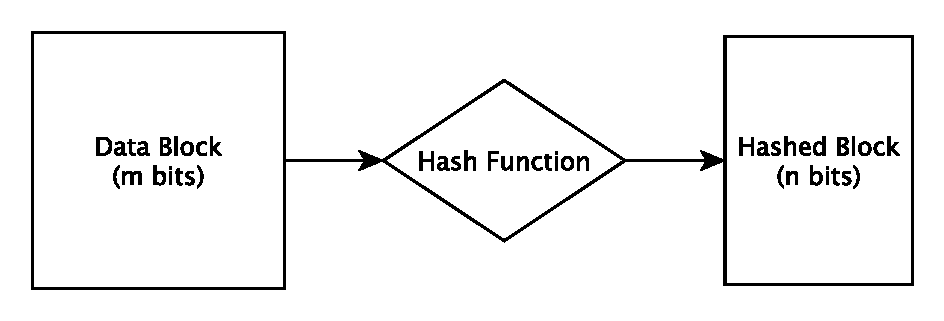
\includegraphics[scale=.6]{IMG/hash2}
\end{figure}
\end{frame}


\begin{frame}
\frametitle{Designing Hash Functions}

We hash a message by sectioning it into blocks of fixed size $m$, say $M_1,\dots, M_k$. Let $S$ be some \textbf{seed value} of size $m$. We compute as follows:
\begin{itemize}
\item $H_1 = H(S, M_1)$
\item $H_2 = H(H_1, M_2)$
\item $\cdots$
\item $H_k = H(H_{k-1}, M_k)$
\end{itemize}
where $H_k$ is the final output, or the hash value. 
\end{frame}

\begin{frame}
\frametitle{Sequential Applications of Hashing}

The following figure illustrates this concept. 
\begin{figure}
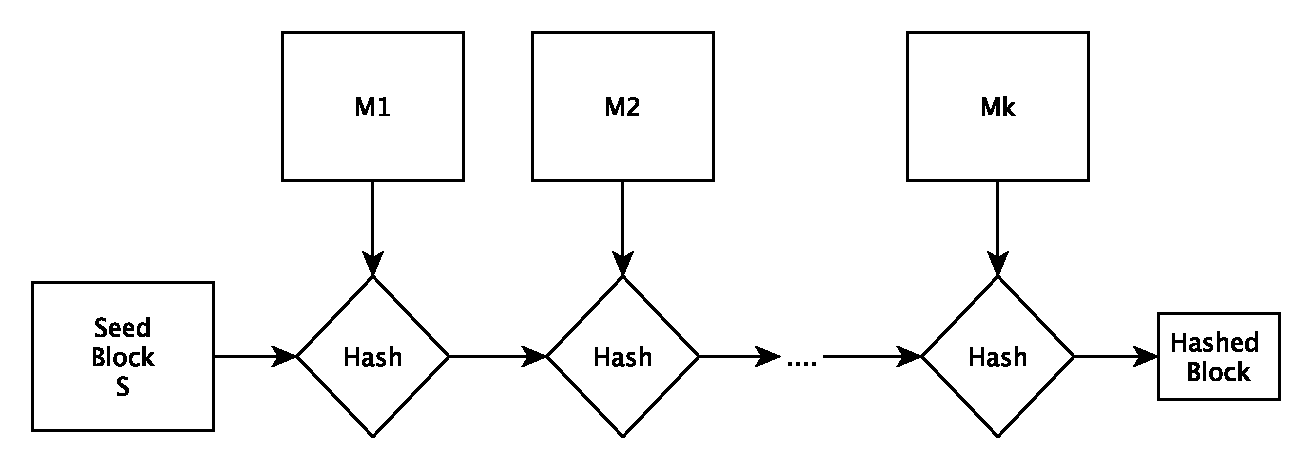
\includegraphics[scale=.5]{IMG/hash3}
\end{figure}

This is known as an \textbf{avalance effect}. The hash of the entire message is the hash of the last block.
\end{frame}


\begin{frame}
\frametitle{Popular Hash Functions}

Will be discussed in more detail next week. 
\begin{itemize}
\item Message Digest (MD)
\item Secure Hash Function (SHA)
\item RIPEMD
\item Whirlpool
\end{itemize}
\end{frame}


\begin{frame}
\frametitle{Hash Values for Password Storage}

Often times, the cleartext value of your password is not what will be stored by a logon server. Instead, the hash of your password is stored. Thus a malicious third party who hacks the database only has access to the hash of your password -- not the password itself. \newline

Due to collision-resistance, this malicious third party should not be able to forge your credentials and long on in your name. 
\end{frame}

\begin{frame}
\frametitle{Password Storage Diagram}

\begin{figure}
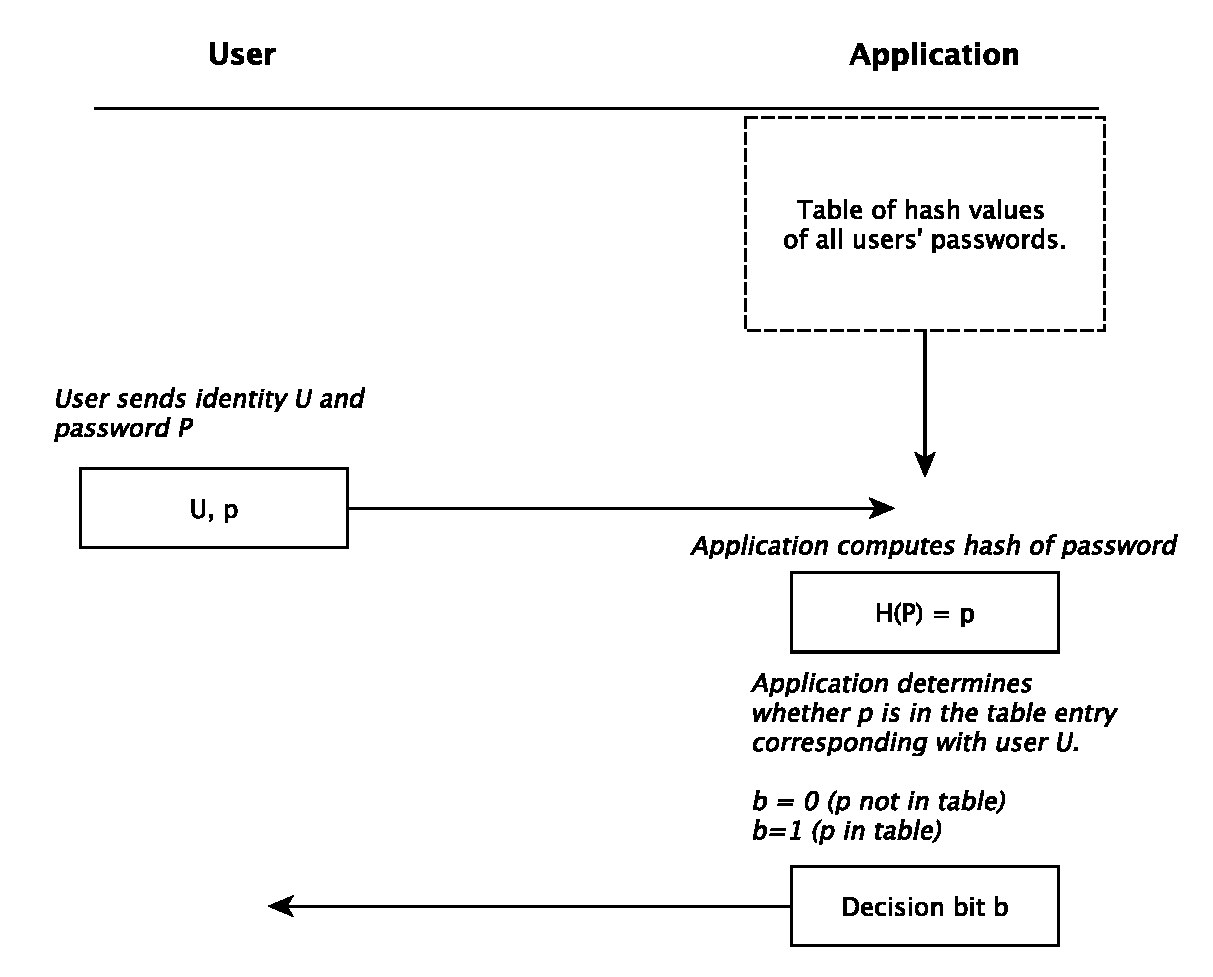
\includegraphics[scale=.45]{IMG/pw}
\end{figure}
\end{frame}


\begin{frame}
\frametitle{Hash Functions for Data Integrity}

Suppose you wish to verify that someone has not modified an original file. 
\includegraphics[scale=.4]{IMG/dic}
Note that the verifier must know independently about the originality of the data. 
\end{frame}


\begin{frame}
\frametitle{Overview of SHA}

We now watch the following video  for a broad overview of SHA. 

\url{https://www.youtube.com/watch?v=5OVb4I5fhKI}
\end{frame}


\begin{frame}
\frametitle{SHA-1}

Let's watch the following video of how SHA1 works.

\url{https://www.youtube.com/watch?v=aLvwpJcOy6s}
\end{frame}

\begin{frame}
\frametitle{References}

\begin{itemize}
\item \emph{Applied Cryptography} By Schneier, Chapter 18
\item \url{https://www.cs.cmu.edu/~guna/15-123S11/Lectures/Lecture17.pdf}
\item \url{https://www.tutorialspoint.com/cryptography/cryptography_hash_functions.htm}
\end{itemize}
\end{frame}
\end{document}


